\chapter{Ergebnisse}
\label{sec:ergebnisse}



\vspace*{-2.5mm}
\renewcommand{\arraystretch}{1.2}
\begin{table}[h!]
	\centering 
	\caption{Messwerttabelle für den Praktikumsversuch Thermische Abfallbehandlung - Grundlagen}
	\resizebox{\textwidth}{!}{
	\begin{tabulary}{23cm}{l|c|c|c}
		\textbf{Daten} & \textbf{Einheit}  & \textbf{Vorher} & \textbf{Nachher} \\ 
		\hline  
	Masse Tiegel (TIC-Probe) & $\si{\gram}$ & 45,717 & 53,0574\\
	Masse TIC-Probe	& $\si{\gram}$ & 38,717 & 7,340\\
	Masse Tiegel (original Abfall)	& $\si{\gram}$ &28,4613 & 29,0690\\
	Masse original Abfall (zur Trocknung) & $\si{\gram}$ &2,976 & 2,878\\
	\cline{3-4}
	Trockensubstanz orginal Abfall & \text{Ma.-\%} & \multicolumn{2}{c}{96,71\%}  \\
	\cline{3-4}
	Masse org. Abfall (zur Verbrennung) & $\si{\gram}$ & 2,878& 0,609\\
	\cline{3-4}
	org. Trockensubstanz original Abfall &\text{Ma.-\%} &\multicolumn{2}{c}{ 79,54\% }  \\
	\hline
	\multicolumn{2}{c|}{\textbf{Messung TIC}}   & \textbf{Masse $\left[ \si{\gram} \right] $} & \textbf{Messergebnis $\left[ \si{\micro \volt
	\per \minute}  \right] $} \\
	\hline
	\multicolumn{2}{l|}{Abfallprobe 1 für TIC-Messung}  & 0,994& 40329,7\\
	\multicolumn{2}{l|}{Kalibrierpunkt 1 ($CaCO_3$)}  & 0,0618& 33472,8\\
	\multicolumn{2}{l|}{Kalibrierpunkt 2 ($CaCO_3$)}  & 0,073& 37642,8\\
	\multicolumn{2}{l|}{Abfallprobe 2 für TIC-Messung}  &0,999 & 55644,0\\
	\hline
	\multicolumn{2}{c|}{\textbf{Messung TC \& Cl}}   & \textbf{Masse $\left[ \si{\gram} \right] $} & \textbf{Messergebnis $\left[ \si{\gram\per\kilogram}\right] $ } \\
	\hline
	\multicolumn{2}{l|}{TC Blindwert (z.B. gebrannter Kalk)}  &0,2343 &4,11 \\
	\multicolumn{2}{l|}{TC orig. Abfall (nach Trocknung)}  &0,0790 & 274,26\\
	\multicolumn{2}{l|}{TC TIC-Mischprobe (nach Trocknung)}  & 0,4749& 43,85\\
	\multicolumn{2}{l|}{Chlorgehalt orig. Abfall (\SI{80}{\milli\liter} aus \SI{160}{\milli\liter})}  & - & 0,855 (0,085\%)\\
	\end{tabulary}
}
	\label{master_messwerttabelle}
\end{table}
\FloatBarrier
\vspace*{-2.5mm}
\renewcommand{\arraystretch}{1.2}

%\begin{table}[h!]
%	\centering 
%	%\resizebox{\textwidth}{!}{
%		\begin{tabulary}{23cm}{L|C|C}
%			\textbf{Messung TIC} & \textbf{Masse $\left[ \si{\gram} \right] $} & \textbf{Messergebnis $\left[ \si{\micro \volt
%					\per \minute}  \right] $} \\
%			\hline
%			Abfallprobe für TIC-Messung  & & \\
%			Kalibrierpunkt 1 ($CaCO_3$)  & & \\
%			Kalibrierpunkt 2 ($CaCO_3$) & & \\
%			%\multicolumn{1}{l}{Kalibrierpunkt 1 ($CaCO_3$)} & & & \\
%			\hline
%			\textbf{Messung TC \& Cl}  & \textbf{Masse $\left[ \si{\gram} \right] $} & \textbf{Messergebnis $\left[ \si{\gram\per\kilogram}\right] $ } \\
%			\hline
%			TC Blindwert (z.B. gebrannter Kalk) & & \\
%			TC orig. Abfall (nach Trocknung) & & \\
%			TC TIC-Mischprobe (nach Trocknung) & & \\
%			Chlorgehalt orig. Abfall %(\SI{80}{\milli\liter} aus \SI{160}{\milli\liter}) 
%			& & \\
%		\end{tabulary}
%	%}
%\end{table}
%\FloatBarrier

\newpage

\section{Bestimmung des TIC-Gehaltes}

Im folgenden Abschnitt sind die Messwerte für die Massen %$\left[\si{\gram}\right]$ 
der Müll- und der Carbonatproben aufgeführt, sowie deren per Software berechnetes Messergebnis $\left[\si{\micro \volt \per \minute}\right]$. Alle Werte für den TIC-Gehalt in Tabelle \ref{master_messwerttabelle} wurden vor der Trocknung der Proben aufgenommen.

%Tabelle Zeiten Start
%\vspace*{-2.5mm}
%\renewcommand{\arraystretch}{1.2}
%\begin{table}[h!]
%	\centering 
%	\caption{Massen (vor Trocknung) und Ergebnisse der Messung}
%	%\resizebox{0.9\textwidth}{!}{ 
%		\begin{tabulary}{23cm}{L|C|C}
%			\textbf{Probe} & \textbf{Masse} $\boldsymbol{m \left[\si{\gram}\right]}$ & \textbf{Messergebnis} $\boldsymbol{e \left[\si{\micro \volt \per \minute}\right]}$\\ 
%			\hline  
%			Abfallprobe für TIC-Messung		& 0,9940  	& 40.329,7\\
%			Abfallprobe für TIC-Messung 2	& 0,9990 	& 55.644,0\\
%			Kalibrierpunkt 1 ($CaCO_3$)		& 0,0618 	& 33.472,8\\
%			Kalibrierpunkt 2 ($CaCO_3$)		& 0,0730 	& 37.642,8\\
%		\end{tabulary}
%\label{tic}
%\end{table}
%\FloatBarrier
%Ende Zeiten Tabelle

\subsubsection{Bestimmung des Carbonatgehaltes $\boldsymbol{\chi}$ für Probe 1}
\begin{flalign}
	 	\frac{m_{\text{Abfall-Carbonat}}}{e_{\text{Abfall-Carbonat}}} &=	\frac{m_{\text{Carbonat}}}{e_{\text{Carbonat}}} \\[5pt]
		m_{\text{Abfall-Carbonat}} 		&= 	\frac{e_{\text{Abfall-Carbonat}}}{e_{\text{Carbonat}}}*m_{\text{Carbonat}}\\[5pt]
		m_{\text{Abfall-Carbonat}} 		&= \frac{\SI{40329,7}{\micro \volt \per \minute}}{\SI{33472,8}{\micro \volt \per \minute}}*\SI{0.0618}{\gram}\\[5pt]
		m_{\text{Abfall-Carbonat}} 		&= \underline{\SI{0.0745}{\gram}}\\[8pt]
		\chi_{\text{Abfall-Carbonat}} 	&= \frac{m_{\text{Abfall-Carbonat}}}{m_{\text{Abfall}}}\\[5pt]
		\chi_{\text{Abfall-Carbonat}} 	&= \frac{\SI{0.0745}{\gram}}{\SI{0.9940}{\gram}}\\[5pt]
		\chi_{\text{Abfall-Carbonat}} 	&= \underline{\underline{0,07494 \approx 7,5 \%}}
\end{flalign}

\subsubsection{Bestimmung des Carbonatgehaltes $\boldsymbol{\chi}$ für Probe 2}
\begin{flalign}
\frac{m_{\text{Abfall-Carbonat}}}{e_{\text{Abfall-Carbonat}}} &=	\frac{m_{\text{Carbonat}}}{e_{\text{Carbonat}}} \\[5pt]
m_{\text{Abfall-Carbonat}} 		&= 	\frac{e_{\text{Abfall-Carbonat}}}{e_{\text{Carbonat}}}*m_{\text{Carbonat}}\\[5pt]
m_{\text{Abfall-Carbonat}} 		&= \frac{\SI{55644,0}{\micro \volt \per \minute}}{\SI{33472,8}{\micro \volt \per \minute}}*\SI{0,0618}{\gram}\\[5pt]
m_{\text{Abfall-Carbonat}} 		&= \underline{\SI{0,1027}{\gram}}\\[8pt]
\chi_{\text{Abfall-Carbonat}} 	&= \frac{m_{\text{Abfall-Carbonat}}}{m_{\text{Abfall}}}\\[5pt]
\chi_{\text{Abfall-Carbonat}} 	&= \frac{\SI{0,1027}{\gram}}{\SI{0.9990}{\gram}}\\[5pt]
\chi_{\text{Abfall-Carbonat}} 	&= \underline{\underline{0,10284 \approx 10,3 \%}}
\end{flalign}

%Start
\begin{figure}[h!]
	\centering
	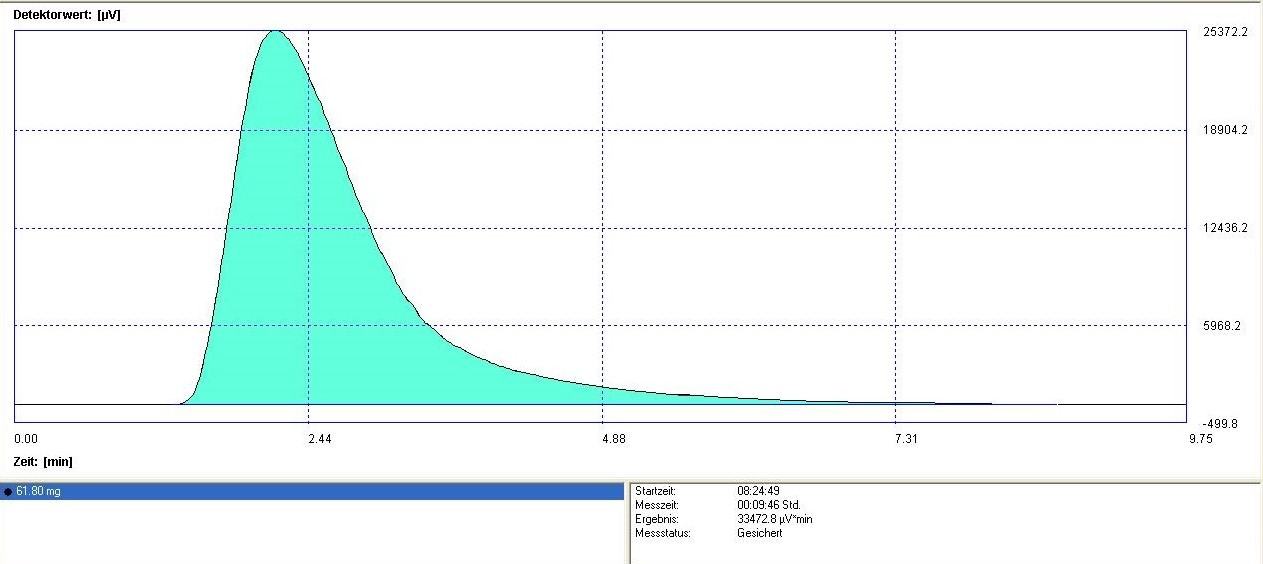
\includegraphics[width=0.6\textwidth]{img/CaCO3_k1}
	\caption{Kalibrierkurve 1 für \ce{CaCO3}}
	\label{dia:k1}
\end{figure}
\FloatBarrier
%Ende

%Start
\begin{figure}[h!]
	\centering
	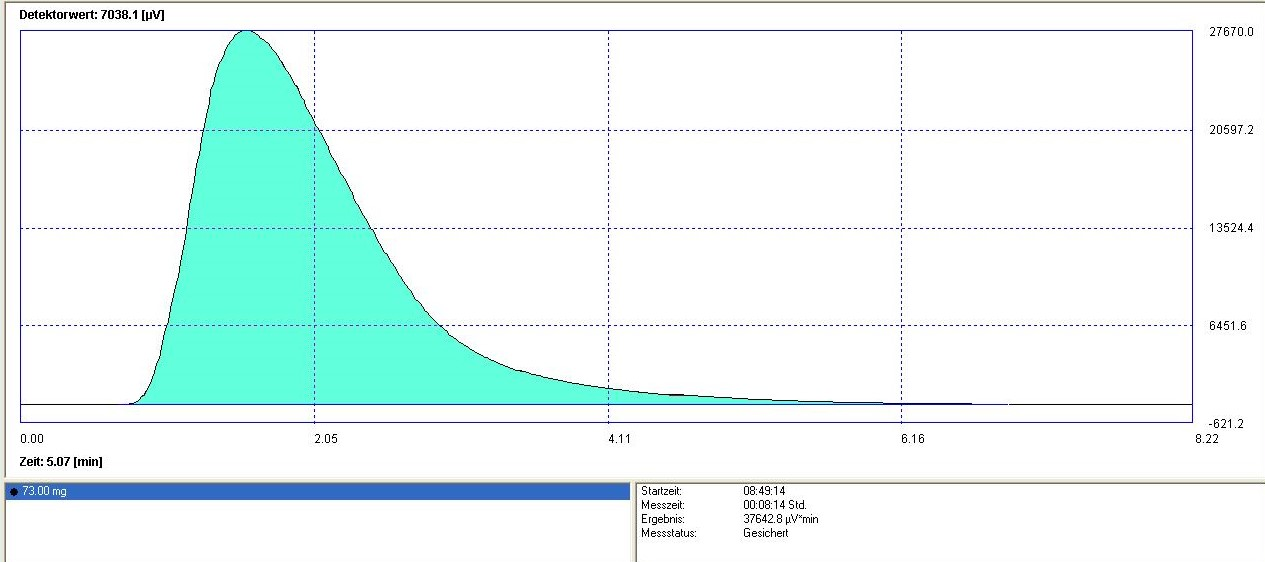
\includegraphics[width=0.6\textwidth]{img/CaCO3_k2}
	\caption{Kalibrierkurve 1 für \ce{CaCO3}}
	\label{dia:k2}
\end{figure}
\FloatBarrier
%Ende

%Start
\begin{figure}[h!]
	\centering
	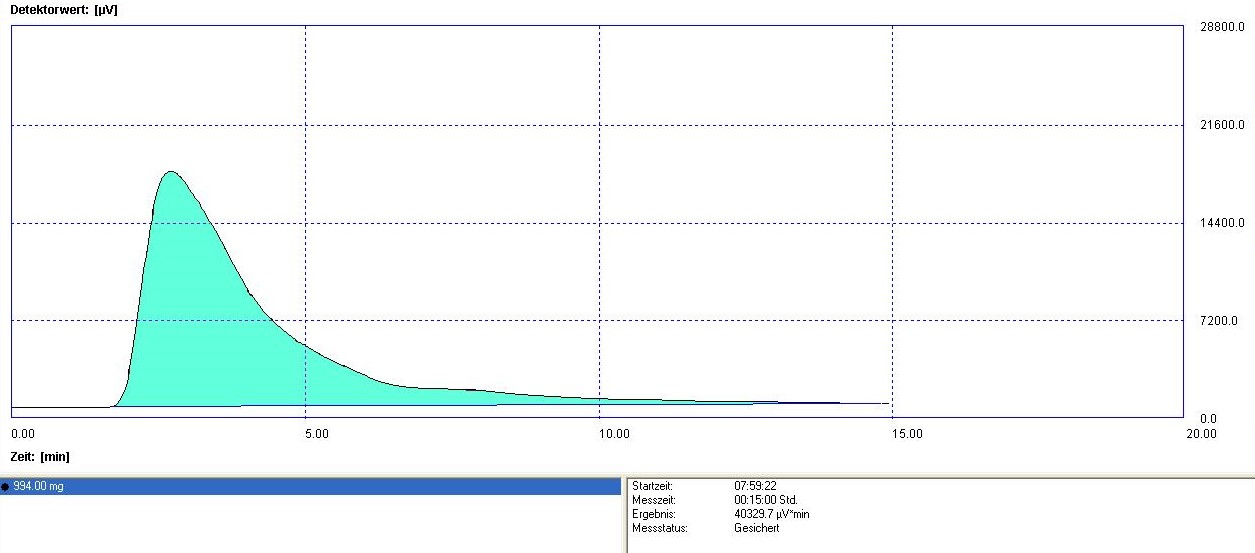
\includegraphics[width=0.6\textwidth]{img/Muell_V1}
	\caption{Messkurve für Müllprobe 1}
	\label{dia:m1}
\end{figure}
\FloatBarrier
%Ende

%Start
\begin{figure}[h!]
	\centering
	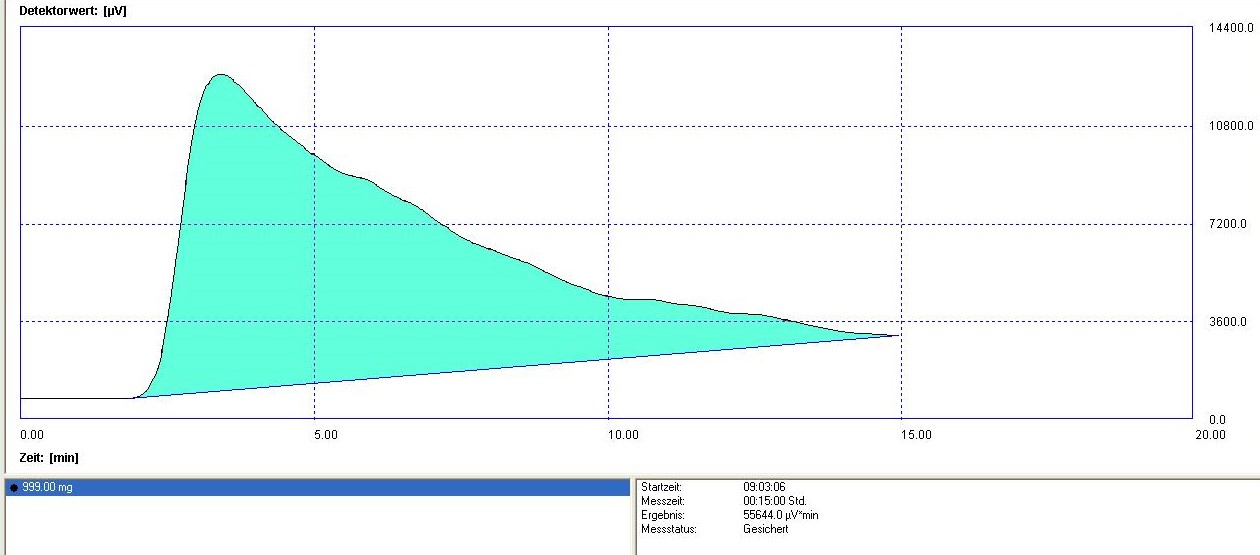
\includegraphics[width=0.6\textwidth]{img/Muell_V2}
	\caption{Messkurve für Müllprobe 2}
	\label{dia:m2}
\end{figure}
\FloatBarrier
%Ende

\newpage

\begin{center}
	\begin{tikzpicture}
	\begin{axis}[
	xlabel={$m \left[\si{\milli \gram}\right]$},
	ylabel={$\Phi \left[\si{\micro \volt \minute}\right]$},
	xmin = 45,
	xmax = 120,
	ymin=20000,
	ymax=70000,
	axis x line=bottom,
	axis y line=left,
	legend style={
		at={(1.1,0.97)},anchor=north west}]
	
	\addplot [domain=0:200, samples=101,dotted]{539.91*x+106.15};
	\addlegendentry{Verlauf der Messdaten};
	%\addplot [domain=0:200, samples=101,dashed]{476.91*x + 3876.1};
	\addplot [domain=0:200, samples=101,]{372.32*x + 10463};
	\addlegendentry{Kalibrierkurve $(372.32*x + 10463)$};
	\addplot+ [mark=*, color=black] coordinates {(74.55,40329.7)};
	\addlegendentry{\ce{CaCO3}-Müllprobe 1};
	\addplot [mark=*, color=black] coordinates {(102.9,55644.0)};
	\addlegendentry{\ce{CaCO3}-Müllprobe 2};
	\addplot [mark=x, color=blue, only marks] coordinates {(61.8,33472.8) (73.0,37642.8)};
	\addlegendentry{\ce{CaCO3}-Blindproben};
	
	\addplot [mark=x, color=red] coordinates {(74.5,40329.7)};
	\addlegendentry{Kalibrierpunkt (berechnet)};
	\end{axis}%
	\end{tikzpicture}%
\end{center}

\subsubsection{Abweichung von Kalibrierkurve}

\begin{flalign}
	a	&= \frac{\Phi_{Mess}-\Phi_{Kali}}{\Phi_{Kali}}\\[2mm]
	a_1	&= \frac{\SI{40329.7}{\micro \volt \minute}-\SI{38219.5}{\micro \volt \minute}}{\SI{38219.5}{\micro \volt \minute}} = \underline{\underline{5,5\%}}\\[2mm]
	a_2	&= \frac{\SI{55644.0}{\micro \volt \minute}-\SI{48773,6}{\micro \volt \minute}}{\SI{48773,6}{\micro \volt \minute}} = \underline{\underline{14,1\%}}
\end{flalign}


\section{Bestimmung des TC-Gehaltes}

\subsubsection{Bestimmung des Trockensubstanzgehalt $\mathbf{TS}$} 
\begin{flalign}
TS \left[\%\right]	&= \frac{m_{\text{Trockensubstanz}}}{m_\text{gesamt}}*100\%\\
TS_{\text{TIC}}		&= \frac{\SI{7,340}{\gram}}{\SI{38,717}{\gram}}*100\%\\
&=\underline{18,96\%}\\[2mm]
TS_{\text{org.}}		&= \frac{\SI{2,878}{\gram}}{\SI{2,976}{\gram}}*100\%\\
&=\underline{96,71\%}
\end{flalign}

\subsubsection{Bestimmung des Wassergehaltes $\mathbf{W}$} 
%Trockensubstanz TIC = 38,717 dann 7,340
%TS original = 2,976 dann 2,878
\begin{flalign}
W \left[\%\right]	&= \frac{m_\text{gesamt}-m_{\text{Trockensubstanz}}}{m_\text{gesamt}}*100\%\\
W_{\text{TIC}}		&= \frac{\SI{38,717}{\gram}-\SI{7,340}{\gram}}{\SI{38,717}{\gram}}*100\%\\
&=\underline{81,04\%}\\[2mm]
W_{\text{org.}}		&= \frac{\SI{2,976}{\gram}-\SI{2,878}{\gram}}{\SI{2,976}{\gram}}*100\%\\
&=\underline{3,29\%}
\end{flalign}

\subsubsection{Bestimmung des Glühverlustes $\mathbf{GV}$}
%VERBENNUNG
\begin{flalign}
GV \left[\%\right]				&= \frac{m_{\text{gesamt}}-m_{\text{Glührückstand}}}{m_\text{gesamt}}*100\%\\[2mm]
GV_{\text{org.}} &= \frac{\SI{2,976}{\gram}-\SI{0,609}{\gram} }{\SI{2,976}{\gram}}*100\%\\
				&= \underline{\SI{79,54}{\percent}}
\end{flalign}

\subsubsection{Bestimmung des Brennwertes $\mathbf{H_s}$}
\begin{flalign}
	H_s \left[\si{\kilo \joule \per \kg}\right]		&= 523*GV^{0,77}\\
	H_s(org.)	&= 523*79,54\%^{0,77}\\	
				&= \underline{\underline{\SI{15203,82}{\kilo \joule \per \kg}\approx\SI{15,20}{\mega \joule \per \kg}\approx\SI{4,2}{\kWh \per \kg}}}
\end{flalign}


\subsubsection{Bestimmung des Heizwertes $\mathbf{H_i}$} 
\begin{flalign}
H_i	\left[\si{\kilo \joule \per \kg}\right]	&= H_s*\frac{TS}{100}-25*\left(0,09*H*TS+W\right)\\
											&= H_s*\frac{TS}{100}-25*\left(0,09*\frac{GV}{15}*TS+W\right)\\[2mm]
H_i(org.)		&= \SI{15203,82}{\kilo \joule \per \kg}*\frac{96,71\%}{100}-25*\left(0,09*\frac{79,54\%}{15}*96,71\%+3,29\%\right)\\
				&= \underline{\underline{\SI{13467,52}{\kilo \joule \per \kg}\approx\SI{13,47}{\mega \joule \per \kg}\approx\SI{3,7}{\kWh \per \kg}}}
\end{flalign}
 